% !TeX TS-program = xelatex

\documentclass[compress, 8pt]{beamer}

\usepackage{presentationtemplate}
\usepackage[askip=3mm, bskip=3mm]{terminal}
\usepackage[linenosfontsize=\tiny, askip=3mm, bskip=3mm]{mylisting}
\usepackage{tcolorbox}
\usepackage{tikz}
\usetikzlibrary{positioning}

\newtcolorbox{task}{
    colback=yellow!50!white,
    boxrule=0.02cm,
    colframe=black,
    sharp corners,
    left=0mm,
    right=0mm,
    top=0mm,
    bottom=0mm,
    before upper={\textbf{Задание}:\:},
}

\title{Указатели и ссылки}

\begin{document}

\frame[plain]{\titlepage}

\begin{frame}[fragile]

    \frametitle{Получение указателя}

    \begin{columns}[T]

        \begin{column}{0.5\textwidth}

            Каждому типу переменной в C++ соответствует тип \textbf{указателя}
            \footnote{\url{https://en.cppreference.com/w/cpp/language/pointer}}
            (pointer) на эту переменную.
            В переменной указателя хранится адрес переменной соответствующего
            типа в оперативной памяти (также говорят, что указатель
            \textbf{ссылается} на переменную).
            Сохранить адрес переменной в указатель можно с помощью оператора \verb|&|.

            \begin{myinplacelisting}[minted language=cpp]
const short s = |\colorbox{green!20}{0x1122}|;
const short* p = &s;
            \end{myinplacelisting}

        \end{column}

        \begin{column}{0.5\textwidth}

            \centering

            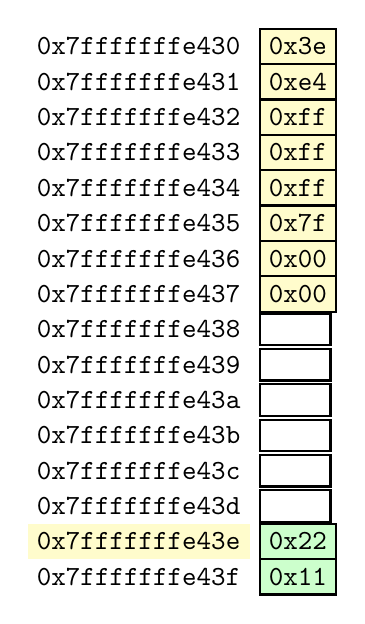
\begin{tikzpicture} [
                bytenode/.style={
                    rectangle,
                    thick,
                    minimum width=9mm,
                    minimum height=4mm
                }
            ]

                \node[bytenode]                 (addr0)                                         {\verb|0x7fffffffe43f|};
                \node[bytenode, fill=yellow!20] (addr1)     [above=-\pgflinewidth of addr0]     {\verb|0x7fffffffe43e|};
                \node[bytenode]                 (addr2)     [above=-\pgflinewidth of addr1]     {\verb|0x7fffffffe43d|};
                \node[bytenode]                 (addr3)     [above=-\pgflinewidth of addr2]     {\verb|0x7fffffffe43c|};
                \node[bytenode]                 (addr4)     [above=-\pgflinewidth of addr3]     {\verb|0x7fffffffe43b|};
                \node[bytenode]                 (addr5)     [above=-\pgflinewidth of addr4]     {\verb|0x7fffffffe43a|};
                \node[bytenode]                 (addr6)     [above=-\pgflinewidth of addr5]     {\verb|0x7fffffffe439|};
                \node[bytenode]                 (addr7)     [above=-\pgflinewidth of addr6]     {\verb|0x7fffffffe438|};
                \node[bytenode]                 (addr8)     [above=-\pgflinewidth of addr7]     {\verb|0x7fffffffe437|};
                \node[bytenode]                 (addr9)     [above=-\pgflinewidth of addr8]     {\verb|0x7fffffffe436|};
                \node[bytenode]                 (addr10)    [above=-\pgflinewidth of addr9]     {\verb|0x7fffffffe435|};
                \node[bytenode]                 (addr11)    [above=-\pgflinewidth of addr10]    {\verb|0x7fffffffe434|};
                \node[bytenode]                 (addr12)    [above=-\pgflinewidth of addr11]    {\verb|0x7fffffffe433|};
                \node[bytenode]                 (addr13)    [above=-\pgflinewidth of addr12]    {\verb|0x7fffffffe432|};
                \node[bytenode]                 (addr14)    [above=-\pgflinewidth of addr13]    {\verb|0x7fffffffe431|};
                \node[bytenode]                 (addr15)    [above=-\pgflinewidth of addr14]    {\verb|0x7fffffffe430|};

                \node[bytenode, draw, fill=green!20]    (b0)    [right=1mm of addr0]    {\verb|0x11|};
                \node[bytenode, draw, fill=green!20]    (b1)    [right=1mm of addr1]    {\verb|0x22|};
                \node[bytenode, draw]                   (b2)    [right=1mm of addr2]    {};
                \node[bytenode, draw]                   (b3)    [right=1mm of addr3]    {};
                \node[bytenode, draw]                   (b4)    [right=1mm of addr4]    {};
                \node[bytenode, draw]                   (b5)    [right=1mm of addr5]    {};
                \node[bytenode, draw]                   (b6)    [right=1mm of addr6]    {};
                \node[bytenode, draw]                   (b7)    [right=1mm of addr7]    {};
                \node[bytenode, draw, fill=yellow!20]   (b8)    [right=1mm of addr8]    {\verb|0x00|};
                \node[bytenode, draw, fill=yellow!20]   (b9)    [right=1mm of addr9]    {\verb|0x00|};
                \node[bytenode, draw, fill=yellow!20]   (b10)   [right=1mm of addr10]   {\verb|0x7f|};
                \node[bytenode, draw, fill=yellow!20]   (b11)   [right=1mm of addr11]   {\verb|0xff|};
                \node[bytenode, draw, fill=yellow!20]   (b12)   [right=1mm of addr12]   {\verb|0xff|};
                \node[bytenode, draw, fill=yellow!20]   (b13)   [right=1mm of addr13]   {\verb|0xff|};
                \node[bytenode, draw, fill=yellow!20]   (b14)   [right=1mm of addr14]   {\verb|0xe4|};
                \node[bytenode, draw, fill=yellow!20]   (b15)   [right=1mm of addr15]   {\verb|0x3e|};

            \end{tikzpicture}

        \end{column}

    \end{columns}

\end{frame}

\begin{frame}[fragile]

    \frametitle{Получение указателя}

    \begin{columns}[T]

        \begin{column}{0.5\textwidth}

            В указатель сохраняется адрес объекта, аллоцированного
            в куче (heap).

            \begin{myinplacelisting}[minted language=cpp]
const short* p
    = new short(|\colorbox{green!20}{0x1122}|);
delete p;
            \end{myinplacelisting}

            Размер указателя на конкретной архитектуре/платформе зависит от
            ширины шины, которая адресует ОЗУ.
            Типичные размеры указателей --- 4Б и 8Б.

        \end{column}

        \begin{column}{0.5\textwidth}

            \centering

            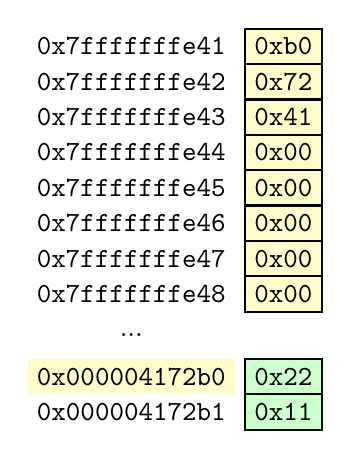
\begin{tikzpicture} [
                bytenode/.style={
                    rectangle,
                    thick,
                    minimum width=9mm,
                    minimum height=4mm
                }
            ]

                \node[bytenode]                     (heapaddr0)                                             {\verb|0x000004172b1|};
                \node[bytenode, fill=yellow!20]     (heapaddr1)     [above=-\pgflinewidth of heapaddr0]     {\verb|0x000004172b0|};
                \node[bytenode, minimum height=6mm] (noaddr)        [above=-\pgflinewidth of heapaddr1]     {...};
                \node[bytenode]                     (stackaddr0)    [above=-\pgflinewidth of noaddr]        {\verb|0x7fffffffe48|};
                \node[bytenode]                     (stackaddr1)    [above=-\pgflinewidth of stackaddr0]    {\verb|0x7fffffffe47|};
                \node[bytenode]                     (stackaddr2)    [above=-\pgflinewidth of stackaddr1]    {\verb|0x7fffffffe46|};
                \node[bytenode]                     (stackaddr3)    [above=-\pgflinewidth of stackaddr2]    {\verb|0x7fffffffe45|};
                \node[bytenode]                     (stackaddr4)    [above=-\pgflinewidth of stackaddr3]    {\verb|0x7fffffffe44|};
                \node[bytenode]                     (stackaddr5)    [above=-\pgflinewidth of stackaddr4]    {\verb|0x7fffffffe43|};
                \node[bytenode]                     (stackaddr6)    [above=-\pgflinewidth of stackaddr5]    {\verb|0x7fffffffe42|};
                \node[bytenode]                     (stackaddr7)    [above=-\pgflinewidth of stackaddr6]    {\verb|0x7fffffffe41|};

                \node[bytenode, draw, fill=green!20]    (b0)    [right=1mm of heapaddr0]    {\verb|0x11|};
                \node[bytenode, draw, fill=green!20]    (b1)    [right=1mm of heapaddr1]    {\verb|0x22|};
                \node[bytenode, draw, fill=yellow!20]   (b8)    [right=1mm of stackaddr0]   {\verb|0x00|};
                \node[bytenode, draw, fill=yellow!20]   (b9)    [right=1mm of stackaddr1]   {\verb|0x00|};
                \node[bytenode, draw, fill=yellow!20]   (b10)   [right=1mm of stackaddr2]   {\verb|0x00|};
                \node[bytenode, draw, fill=yellow!20]   (b11)   [right=1mm of stackaddr3]   {\verb|0x00|};
                \node[bytenode, draw, fill=yellow!20]   (b12)   [right=1mm of stackaddr4]   {\verb|0x00|};
                \node[bytenode, draw, fill=yellow!20]   (b13)   [right=1mm of stackaddr5]   {\verb|0x41|};
                \node[bytenode, draw, fill=yellow!20]   (b14)   [right=1mm of stackaddr6]   {\verb|0x72|};
                \node[bytenode, draw, fill=yellow!20]   (b15)   [right=1mm of stackaddr7]   {\verb|0xb0|};

            \end{tikzpicture}

        \end{column}

    \end{columns}

\end{frame}

\begin{frame}[fragile]

    \frametitle{Разыменование указателя}

    \hfill \break

    Разыменованием указателя называется получение значения, адрес которого
    хранится в указателе.
    Разыменование осуществляется при помощи оператора \verb|*|.

    \myinputlisting[minted language=cpp]
        {Presentations/07-Pointers-and-References/deref/}
        {main.cpp}

    \begin{terminalwindow}
!\shellcommand{g++ main.cpp -o main}!
!\shellcommand{./main}!
d=3.14
*p=3.14
    \end{terminalwindow}

\end{frame}

\begin{frame}[fragile]

    \frametitle{Разыменование указателя}

    \hfill \break

    С помощью разыменования указателя возможно изменение объекта,
    на который он ссылается.

    \myinputlisting[minted language=cpp]
        {Presentations/07-Pointers-and-References/deref-and-change/}
        {main.cpp}

    \begin{terminalwindow}
!\shellcommand{g++ main.cpp -o main}!
!\shellcommand{./main}!
d=2.718
    \end{terminalwindow}

\end{frame}

\begin{frame}[fragile]

    \frametitle{Разыменование указателя}

    \begin{task}
        Определите, что выведет программа на листинге.
    \end{task}

    \begin{myinplacelisting}[minted language=cpp]
#include <iostream>

int main() {
    int a = 1;
    int b = a;
    int* p = &b;
    (*p)++;
    std::cout << a << std::endl;
}
    \end{myinplacelisting}

\end{frame}

\begin{frame}[fragile]

    \frametitle{Константные указатели и \\ указатели на константные объекты}

    Константные указатели на неконстантные объекты:

    \begin{itemize}
        \item \textbf{нельзя} менять адрес, который они хранят;
        \item \textbf{можно} менять объект по этому адресу.
    \end{itemize}

    \begin{myinplacelisting}[minted language=cpp]
int a {};
int b {};
int* |\colorbox{yellow}{const}| p = &a;
p = &b; // compilation error
*p = 1; // ok, a == 1
    \end{myinplacelisting}

    \begin{task}
        Найдите ошибку компиляции в коде на листинге и объясните ее.
    \end{task}

    \begin{myinplacelisting}[minted language=cpp]
const int c {};
int* const p1 = &c;
    \end{myinplacelisting}

\end{frame}

\begin{frame}[fragile]

    \frametitle{Константные указатели и \\ указатели на константные объекты}

    Неконстантные указатели на константные объекты:

    \begin{itemize}
        \item \textbf{нельзя} менять объект, на который они указывают;
        \item \textbf{можно} менять адрес, который они хранят.
    \end{itemize}

    \begin{myinplacelisting}[minted language=cpp]
int a {};
int b {};
|\colorbox{yellow}{const}| int* p = &a;
p = &b; // ok, p points to b
*p = 1; // compilation error
    \end{myinplacelisting}

    Константные указатели на константные объекты:

    \begin{itemize}
        \item \textbf{нельзя} менять объект, на который они указывают;
        \item \textbf{нельзя} менять адрес, который они хранят.
    \end{itemize}

    \begin{myinplacelisting}[minted language=cpp]
int a {};
int b {};
|\colorbox{yellow}{const}| int* |\colorbox{yellow}{const}| p = &a;
p = &b; // compilation error
*p = 1; // compilation error
    \end{myinplacelisting}

\end{frame}

\begin{frame}[fragile]

    \frametitle{Константные указатели и \\ указатели на константные объекты}

    \begin{task}
        Найдите ошибки компиляциии и времени выполнения в коде на листингах ниже.
    \end{task}

    \begin{columns}[T]

        \begin{column}{0.5\textwidth}

            \begin{myinplacelisting}[minted language=cpp]
#include <iostream>

void print_ptr(int* p) {
    std::cout << *p
        << std::endl;
}

int main() {
    const int* p = new int{};
    print_ptr(p);
}
            \end{myinplacelisting}

        \end{column}

        \begin{column}{0.5\textwidth}

            \begin{myinplacelisting}[minted language=cpp]
#include <iostream>

int main() {
    int a {};
    const int* const p = &a;
    int* const* const pp = &p;
    **pp = -1;
    std::cout << a
        << std::endl;
}
            \end{myinplacelisting}

        \end{column}

    \end{columns}

\end{frame}

\begin{frame}[fragile]

    \frametitle{Нулевой указатель}

    \hfill \break

    Указатели каждого типа имеют специaльное значение, называемое
    \textbf{нулевым указателем}.
    Обычно при помощи нулевого указателя выражают отсутствие какого-либо
    значения или состояние ошибки.

    Начиная со стандарта C++11, в языке есть ключевое слово \verb|nullptr|,
    которое рекомендуется\footnotemark{} использовать вместо \verb|0|.

    \footnotetext{\url{https://isocpp.github.io/CppCoreGuidelines/CppCoreGuidelines\#Res-nullptr}}

    \begin{myinplacelisting}[minted language=cpp]
const int* pi {};
const char* const pc { nullptr; }
double* pd = 0;
    \end{myinplacelisting}

    Для проверки указателя на \verb|nullptr| возможно воспользоваться
    неявным приведением к типу \verb|bool|
    \footnote{\url{https://isocpp.github.io/CppCoreGuidelines/CppCoreGuidelines\#es87-dont-add-redundant--or--to-conditions}}.

    \begin{myinplacelisting}[minted language=cpp]
const int* const p = get_pointer();
if (!p) {
    std::cout << "got a null pointer" << std::endl;
}
    \end{myinplacelisting}

\end{frame}

\begin{frame}[fragile]

    \frametitle{Нулевой указатель}

    Разыменование указателя для чтения или записи является неопределенным
    поведением и приведет к аварийному завершению работы программы на
    большинстве платформ
    \footnote{\url{https://isocpp.github.io/CppCoreGuidelines/CppCoreGuidelines\#es65-dont-dereference-an-invalid-pointer}}.

    \myinputlisting[minted language=cpp]
        {Presentations/07-Pointers-and-References/null-ptr-deref/}
        {main.cpp}

    \begin{terminalwindow}
!\shellcommand{g++ main.cpp -o main && ./main}!
Segmentation fault (core dumped)
    \end{terminalwindow}

\end{frame}

\begin{frame}[fragile]

    \frametitle{Нулевой указатель}

    \hfill \break

    \myinputlisting[minted language=cpp]
        {Presentations/07-Pointers-and-References/getenv/}
        {main.cpp}

    \begin{terminalwindow}
!\shellcommand{g++ main.cpp -o main}!
!\shellcommand{./main}!
'MY_ENV_VAR' is not defined
!\shellcommand{MY\_ENV\_VAR="hello" ./main}!
'MY_ENV_VAR'=hello
    \end{terminalwindow}

\end{frame}

\begin{frame}[fragile]

    \frametitle{Нулевой указатель}

    \begin{task}
        Найдите ошибку в программе.
    \end{task}

    \begin{myinplacelisting}[minted language=cpp]
#include <iostream>
#include <cstdlib>
#include <string>

int main() {
    const char* envVar {};
    do {
        std::cout << "Enter environment variable: ";
        std::string envVarName {};
        std::cin >> envVarName;
        envVar = std::getenv(envVarName.c_str());
        std::cout << *envVar << std::endl;
    }
    while(envVar);
}
    \end{myinplacelisting}

\end{frame}

\begin{frame}[fragile]

    \frametitle{Арифметика указателей}

    \hfill \break

    Над указателями определены арифметические операции сложения и вычитания.
    Увеличение указателя на \verb|1| "смещает" адрес на размер объекта
    (в байтах), на который он ссылается.
    То же верно и для уменьшения на \verb|1|.

    \myinputlisting[minted language=cpp]
        {Presentations/07-Pointers-and-References/ptr-arithmetic/}
        {main.cpp}

    \begin{terminalwindow}
!\shellcommand{g++ main.cpp -o main && ./main}!
p = 0x7fff5e0dd8c0, (p + 1) = 0x7fff5e0dd8c8
!\shellcommand{./main}!
p = 0x7ffd6cd3aa20, (p + 1) = 0x7ffd6cd3aa28
    \end{terminalwindow}

\end{frame}

\begin{frame}[fragile]

    \frametitle{Арифметика указателей}

    Арифметика указателей неприменима к указателю типа \verb|void|!

    \myinputlisting[minted language=cpp]
        {Presentations/07-Pointers-and-References/void-ptr/}
        {main.cpp}

    \begin{terminalwindow}
!\shellcommand{g++ main.cpp}!
main.cpp: In function ‘int !\textcolor{teal}{main}!()’:
main.cpp:3:5: !\textcolor{orange}{warning}!: ISO C++ forbids incrementing a pointer of type ‘void*’ [!\textcolor{orange}{-Wpointer-arith}!]
    3 |     !\textcolor{orange}{p}!++;
      |     !\textcolor{orange}{\^{}}!
    \end{terminalwindow}

\end{frame}

\begin{frame}[fragile]

    \frametitle{Висячие указатели}

    Указатели, ссылающиеся на объекты с истекшим временем жизни,
    называются \textbf{висячими} (dangling).
    Чтение и запись памяти, на которую они ссылаются, является неопределенным
    поведением
    \footnote{\url{https://github.com/Nekrolm/ubbook/blob/master/lifetime/use\_after\_free\_in\_general.md}}.

    \begin{myinplacelisting}[minted language=cpp]
#include <iostream>

int* get_ptr() {
    int x {};
    return &x;
}

int main() {
    int* const p = get_ptr();
    std::cout << *p // undefined behaviour
        << std::endl;
}
    \end{myinplacelisting}

\end{frame}

\begin{frame}[fragile]

    \frametitle{Висячие указатели}

    В отличие от нулевого указателя, отличить висячий указатель от
    "корректного" практически невозможно.
    Рекомендуется записывать \verb|nullptr| в указатель, который ссылается
    на объект с истекшим времени жизни.
    Это может помочь избежать уязвимости use-after-free
    \footnote{\url{https://owasp.org/www-community/vulnerabilities/Using\_freed\_memory}}.

    \begin{task}
        Найдите проблемы в коде на листинге ниже.
    \end{task}

    \begin{myinplacelisting}[minted language=cpp]
void foo(const int* p);

int main() {
    const int* p1 = new int;
    const int* p2 = p1;
    delete p1;
    p1 = nullptr;
    foo(p2);
}
    \end{myinplacelisting}

\end{frame}

\begin{frame}[fragile]

    \frametitle{Ссылки}

    Альтернативой указателю для хранения адреса объекта является
    \textbf{ссылка}\footnotemark{} (reference).
    Ссылки проще в "использовании" и безопаснее с точки зрения работы с памятью,
    но накладывают следующие ограничения:

    \footnotetext{\url{https://en.cppreference.com/w/cpp/language/reference}}

    \begin{itemize}
        \item Ссылка не может быть инициализирована по-умолчанию.
        \item Адрес объекта, на который ссылается ссылка, нельзя изменить
            (ссылки ведут себя как константные указатели).
        \item Для ссылок отсутствует аналог нулевого указателя.
    \end{itemize}

    \hfill \break

    Ссылки предпочтительнее указателей, когда отсутствие значения невозможно
    или не должно быть возможно.

\end{frame}

\begin{frame}[fragile]

    \frametitle{Инициализация и разыменование ссылок}

    \hfill \break

    Ниже приведены корректные и некорректные примеры инициализации
    и разыменования ссылок.

    \begin{myinplacelisting}[minted language=cpp]
#include <iostream>

int main() {
    int& r {}; // compilation error

    int x {-1};
    int& rx { x }; // ok, rx points to x
    std::cout << rx << std::endl; // prints -1
    rx = -2;
    std::cout << x << std::endl; // prints -2

    const int y {};
    int& ry { y }; // compilation error
    const int& ry { y }; // ok, ry points to y
    ry = -1; // compilation error
}
    \end{myinplacelisting}

\end{frame}

\begin{frame}[fragile]

    \frametitle{Висячие ссылки}

    \begin{task}
        Объясните, почему ссылка в программе --- висячая.
    \end{task}

    \begin{myinplacelisting}[minted language=cpp]
#include <iostream>

void foo(const int* const p) {
    std::cout << *p << std::endl;
    delete p;
}

int main() {
    const int* p = new int{100};
    const int& r { *p };
    foo(p);
    p = nullptr;
}
    \end{myinplacelisting}

\end{frame}

\end{document}
